\documentclass[12pt]{article}
\usepackage{authblk}
\usepackage[margin=2cm]{geometry}
\usepackage[table,xcdraw]{xcolor}
\usepackage{booktabs}
\usepackage{bookmark}
\usepackage{longtable}
\usepackage{rotfloat}
\usepackage{makecell}
\usepackage{graphicx}
\usepackage{float}
\usepackage{subfigure}
\usepackage{url}
\usepackage{mathtools}
\usepackage{amssymb,amsmath,amsthm,amsfonts} 
\usepackage[no-math]{fontspec} 
\usepackage{mathspec}
\usepackage{xunicode} 
\usepackage{xltxtra} 
\defaultfontfeatures{Scale=1.0, Mapping=tex-text}
\newcommand*{\QEDA}{\null\nobreak\hfill\ensuremath{\square}}%
\usepackage{tikz}
% \usepackage[hidelinks]{hyperref}
\usepackage{xeCJK}
\usepackage{fontspec}
\usepackage{setspace}
\usepackage{fancyhdr}
\usepackage{titling}
\usepackage{caption}
\usepackage{enumerate}
\usepackage[shortlabels]{enumitem}
\usepackage{multirow}

\setmainfont{Minion Pro}
\setmathfont{Minion Pro}
\setCJKmainfont{宋體-繁}
\renewcommand{\baselinestretch}{1.35}
\newcommand{\upcite}[1]{\textsuperscript{\textsuperscript{\cite{#1}}}}
% \setlength{\droptitle}{5cm}
% \pagenumbering{gobble} %This eliminate page numbers
\pagestyle{fancy}
\fancyhf{}
\fancyhead[LE,RO]{B09704016, 經濟三張茗傑}
\fancyhead[RE,LO]{Labor Economics (I) PS1}
\rfoot{\thepage}

\setlength{\headheight}{13pt}
\geometry{a4paper,left=1.75cm,right=1.75cm,top=2.75cm,bottom=2cm}
\begin{document}

\section{Programming Setup}

\subsection{Set up DataCamp}
I finished "Introduction to R" course on the DataCamp.

\subsection{R}
The markdown file and the pdf file are here\href{https://github.com/JayChang426/ECON-7069.git}.\label{web} Please find it in folder "PS1."

\subsection{Debugger} \label{1.3}
The R script is also here\href{https://github.com/JayChang426/ECON-7069.git}.\label{web} Please find it in folder "PS1."

\subsection{Setup Github}
The repository is here\href{https://github.com/JayChang426/ECON-7069.git}, \label{web}
including the rmd, pdf, and the R script for \ref{1.3} and \ref{4.2}.

\section{Sign up NBER working paper series}
\begin{enumerate}
    \item The title of the second paper listed on the NBER weekly working paper series that I most recently received is "A Human Capital Theory of Who Escape the Grasp of the Local Monopsonists."
    \item I download the paper "Trade Diversion and Trade Deficits: The Case of the Korea-U.S. Free Trade Agreement", which interests me.
\end{enumerate}

\section{Sign up SRDA}
I downloaded the 2020 PSFD, and here's the graph.
\begin{figure}[H]
    \centering
    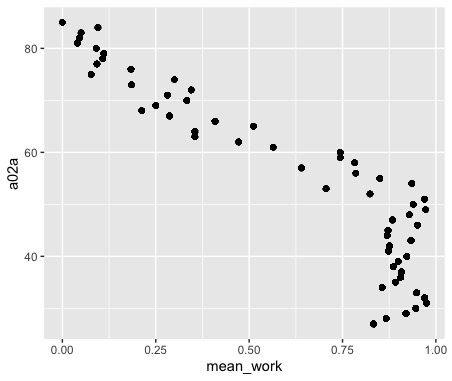
\includegraphics[width=0.4\textwidth]{rate of working against age.jpeg}
\end{figure}

\section{Roy Model}

\subsection{Review}
\begin{enumerate}[1.]
    \item We derive the equations as follows. \begin{flalign}
    \mathbb{E}\ [w_0 | I] & = \mu_0 + \mathbb{E}\ [\varepsilon_0 | \frac{v}{\sigma_v} > Z]& \nonumber \\
                        & = \mu_0 + \sigma_0 \mathbb{E}\ [\frac{\varepsilon_0}{\sigma_0} | \frac{v}{\sigma_v} > Z]& \nonumber \\ 
                        & = \mu_0 + \sigma_0 \mathbb{E}\ [\ \mathbb{E}\ (\frac{\varepsilon_0}{\sigma_0} | \frac{v}{\sigma_v}) | \frac{v}{\sigma_v} > Z]& \\
                        & = \mu_0 + \sigma_0 \rho_{0v} \mathbb{E}\ [\frac{v}{\sigma_v} | \frac{v}{\sigma_v} > Z]& \\ 
                        & = \mu_0 + \sigma_0 \rho_{0v} (\frac{\phi(z)}{1 - \Phi{z}})& \nonumber \\ 
                        & = \mu_0 + \sigma_0 \frac{\sigma_{0v}}{\sigma_0 \sigma_v} (\frac{\phi(z)}{1 - \Phi{z}})& \nonumber \\
                        & = \mu_0 + \frac{\sigma_{0v}}{\sigma_v} (\frac{\phi(z)}{1 - \Phi{z}})& \nonumber \\
                        & = \mu_0 + \frac{\sigma_{01} - {\sigma_{0}}^2}{\sigma_v} (\frac{\phi(z)}{1 - \Phi{z}})& \nonumber \\
                        & = \mu_0 + \frac{\sigma_0 \sigma_1}{\sigma_v} (\frac{\sigma_{01}}{\sigma_{0}\sigma{1}} - \frac{\sigma_0}{\sigma_1}) (\frac{\phi(z)}{1 - \Phi{z}})& \nonumber \\
                        & = \mu_0 + \frac{\sigma_0 \sigma_1}{\sigma_v} (\rho_{01} - \frac{\sigma_0}{\sigma_1})& \nonumber
    \end{flalign}
    Note that from (1) to (2) need to be further explained. First, let $s = \frac{v}{\sigma_v} \thicksim N(0,1).$ Then 
    \begin{flalign*}
    \mathbb{E}\ (\frac{\varepsilon_0}{\sigma_0} | \frac{v}{\sigma_v}) = \frac{1}{\sigma_0}\ \mathbb{E}\ (\varepsilon_0 | s) = \frac{1}{\sigma_0} \frac{\sigma_{0s}}{{\sigma_s}^2}s = \frac{1}{\sigma_0} \frac{\frac{\sigma_{0v}}{\sigma_v}}{1} \frac{v}{\sigma_v} = \rho_{0v} \frac{v}{\sigma_v}
    \end{flalign*}
    Similarly, we can derive $\mathbb{E}\ [w_1 | I] = \mu_1 + \frac{\sigma_1 \sigma_0}{\sigma_v}(\frac{\sigma_1}{\sigma_0} - \rho_{01}) (\frac{\phi(z)}{1 - \Phi{z}})$ \QEDA
    \item If $Q_0 > 0$ and $Q_1 < 0$, then it must be the case that $\rho > \frac{\sigma_0}{\sigma_1}$ and $\rho > \frac{\sigma_1}{\sigma_0}$. No matter $\sigma_0 > \sigma_1$, $\sigma_0 < \sigma_1$ or even $\sigma_0 = \sigma_1$, $\rho > 1$ in one of the inequalities, which is not possible.
\end{enumerate}

\subsection{Simulation} \label{4.2}
The R script of this simulation is also here\href{https://github.com/JayChang426/ECON-7069.git}.\label{web} Please find it in folder "PS1".
The result of 5. and 6. are quite similar, which is not surprising. All other questions are answered in the R script.

\section{Roy Model is Everywhere}
\begin{enumerate}[1. ]
    \item We want to examine the effect of join WTO or not on trade volumes.
    \item We conside the following Roy model for our WTO discussing. \begin{flalign*}
    trade_0 & = \mu_0 + \varepsilon_0& \nonumber \\
    trade_1 & = \mu_1 + \varepsilon_1& \nonumber
    \end{flalign*}
    where joining WTO is 1, not joining WTO is 0.
\end{enumerate}

\end{document}